\chapter{Machine Learning}
Los datos son una fuente de valor por lo que analizarlos y tomar decisiones en función a estos se ha
convertido en algo esencial. Cada vez son más las compañías autodenominadas 
\textit{data-driven company}\index{Data-driven company}, es decir, empresas que toman decisiones de 
futuro e inversión en función al análisis que hacen de sus datos.\\
El \textit{machine learning} se nutre de los datos ya que permite construir modelos sobre estos,
que posteriormente se usarán para tomar dichas decisiones de futuro de la compañía. A modo de ejemplo, estas
decisiones pueden ser: ¿Dónde construir un nuevo centro de datos?, ¿Cómo me anticipo a la posible baja de un
cliente de mis servicios móviles?, ¿Cómo minimizo el coste de mantenimiento de las infraestructuras?...\\
Por estas y más razones, el \textit{machine learning} y las grandes cantidades de datos manejadas en el 
\textit{Big Data} están estrechamente relacionadas.

\section{¿Qué es el machine learning?}
El \textit{Machine Learning}\index{Machine Learning} (ML) es una rama de la inteligencia artificial (IA) 
que se centra en desarrollar métodos para hacer posible que los sistemas aprendan sin ser programados 
explícitamente para ello.
El denominado aprendizaje automático se basa en los datos de entrada o datos de entrenamiento, que
son utilizados para ajustar los modelos tanto predictivos, como clasificatorios o de clusterización.\\
Podemos clasificar los modelos de \textit{machine learning} en dos clases:
\begin{itemize}
  \item \textbf{Aprendizaje supervisado}\index{Aprendizaje!supervisado}: los datos de entrada del 
  algoritmo van etiquetados con la salida esperada, es decir, cada dato de entrada lleva consigo 
  la clase a la que pertenece. De esta manera se pretende que el algoritmo sea capaz de identificar 
  patrones entre los datos de una misma clase para que cuando vea un dato sin etiquetar, este sea 
  capaz de asignarle una clase en función de los patrones aprendidos en la fase de entrenamiento.
  Unos ejemplos de esta clase de algoritmos serían: regresión lineal, regresión logística, 
  \textit{support vector machine}, redes neuronales...
  
  \item \textbf{Aprendizaje no supervisado}\index{Aprendizaje!no supervisado}: los datos pasados 
  al algoritmo no llevan asignados una etiqueta, es el propio algoritmo el que debe aprender 
  patrones similares entre todo el conjunto de datos de entrada.\\
  Algunos ejemplos de aprendizaje no supervisado serían: \textit{KMeans}, \textit{Principal Component Analysis}, 
  \textit{k-nearest neighbors}...
\end{itemize}

Aunque el concepto de \textit{machine learning} apareció a mediados del siglo $XX$, es ahora cuando su evolución
ha crecido en importancia debido al aumento de la capacidad de computo de los ordenadores.
Lo esencial en \textit{machine learning} son los datos, los modelos se alimentan de ellos y es por lo que cuantos más
datos tengamos a disposición, más preciso será nuestro modelo entrenado a coste de un mayor
tiempo de procesamiento (\cite{DBLP:books/lib/Bishop07}). Esta afirmación es matizable, ya que en ciertos casos 
(ver: \url{https://en.wikipedia.org/wiki/Bias%E2%80%93variance_tradeoff})
la inclusión de más datos a tu algoritmo no aumentara su desempeño.
\newline

El ML tiene campos de aplicación muy diversos tales como procesamiento del lenguaje natural, robótica,
desarrollo de motores de búsqueda y recomendación, detección de fraude...\\

\section[\textit{Machine Learning} distribuido]{¿Por qué desarrollar \textit{machine learning} de manera distribuida?}
En la era de la generación masiva de datos, el mejor aliado del \textit{Big Data} es el \textit{machine learning}.
Gracias a esto podemos generar modelos artificiales en muy diversas áreas para sacar un beneficio
mayor a nuestros datos. Podemos crear modelos predictivos, probabilísticos, clasificatorios,
sistemas de detección de fraude y anomalías, algoritmos de compresión de datos...
\newline

Para entrenar estos modelos necesitamos datos, tradicionalmente, este proceso de entrenamiento
del algoritmo se hacía de manera secuencial en una sola máquina. Hay muchos lenguajes de programación, 
librerías y herramientas para llevar a cabo este proceso de entrenamiento y modelización como por
ejemplo \textit{R}, \textit{Matlab}, \textit{Octave} o \textit{Python} mediante la librería 
\href{http://scikit-learn.org/stable/}{\textit{sklearn}}.
Estas herramientas funcionan muy bien pero solo en conjuntos pequeños de datos.
\newline

Si queremos desarrollar un modelo con un buen rendimiento necesitamos muchos datos, tantos que a veces
superan ampliamente la memoria disponible del ordenador así como la capacidad de los procesadores para
poder procesar toda la información en un tiempo razonable.\\
A medida que el conjunto de datos de entrenamiento crece, las herramientas tradicionales se quedan
inservibles para este propósito, por esta razón, estamos en la necesidad de desarrollar algoritmos
paralelos que den solución a estos problemas.
\newline

En el artículo de investigación \cite{NIPS2006_3150}, se puede comprobar los efectos de la paralelización
(en cuanto a términos de rendimiento) de algunos algoritmo de \textit{machine learning}. Esto pone de
manifiesto más aún si cabe la necesidad de distribuir los cómputos entre varias máquinas. Como se ve en
la \autoref{sec:ml_pipeline}, el proceso de creación de un modelo de \textit{machine learning} se basa en
la prueba y error por lo que normalmente es necesario entrenar el modelo sobre el mismo conjunto de datos
varias veces, hasta que se obtengan las métricas deseadas. Esto aumenta más aún si cabe el tiempo necesario
de entrenamiento, que en entornos secuenciales pueden llegar a ser inviables.
\newline

En el \autoref{chap:implementacion_paralela} se estudiará, analizará e implementará de manera paralela 
algunos de los algoritmos más populares y usados hoy en día de \textit{machine learning}.

\section{Machine learning pipelines}\label{sec:ml_pipeline}
El desarrollo de un modelo de \textit{machine learning} pasa por una serie de fases o procesos de desarrollo,
desde el preprocesamiento de los datos crudos hasta la utilización de dicho modelo en un entorno
de producción.

En la vida real los datos provienen de diversas fuentes como sensores, redes sociales o bases de datos.
Estos datos no siempre vienen formateados de manera numérica por lo que
hay diversos motivos por los cuales el preprocesamiento es algo fundamental.\\
Nos podemos encontrar con que nos faltan valores en un determinado registro y una determinada columna
que deben ser rellenados o eliminados con el fin de utilizarlos posteriormente en nuestro modelo.
En los datos crudos suele ser muy común encontrarse con características que son categóricas en 
vez de numéricas, esto es, un registro puede contener el sexo de una persona (hombre, mujer), el color 
de un coche (rojo, negro, azul...). 
Todas estas características deben ser convertidas a un formato numérico (escalar o vector de escalares) 
para ser procesadas posteriormente.\\
También puede ser que nuestro \textit{dataset} crudo tal vez contenga 
\textit{outliers}\index{Outlier}\footnote{los outliers son valores atípicos  respecto al resto de observaciones 
de una muestra.} que queramos eliminar o transformar, etc.
\newline

Debido a estos motivos, necesitamos un preprocesamiento de los datos con el fin de limpiarlos y 
prepararlos para ser consumidos por el modelo matemático.\\
Posteriormente, en la mayoría de los casos es necesario escalar los datos para un desempeño óptimo, 
debido a que si no lo hacemos, las características de los datos con un valor numérico más alto 
tendrán más peso en la función objetivo. Este escalado previo es necesario en modelos como 
las redes neuronales o la regresión logística.

\clearpage

\noindent De manera esquemática, los pasos a seguir son:
\begin{framed}
\begin{enumerate}
  \item \textbf{Preprocesamiento}
  \begin{enumerate}
    \item Limpieza y purga: quitar o rellenar registros vacíos, tratamiento de valores nulos 
          y $N/A$, convenciones en formato de fechas...
    \item \textit{Feature Engineering}\index{Feature engineering}: convertir variables categóricas a numéricas, 
          estandarización o escalado de los datos...
    \item División de los datos: dividir el conjunto de datos en conjunto de entrenamiento y 
          conjunto de test (generalmente en proporciones $70 - 30\%$ o similar).
  \end{enumerate}
  
  \item \textbf{Procesamiento}
  \begin{enumerate}
    \item Elección de modelo que mejor se ajuste a nuestro problema 
          (\textit{Support Vector Machine}, Redes Neuronales, regresión lineal, etc.)
    \item Entrenamiento: \textit{Hyperparameter tuning}\index{Hyperparameter tuning}, 
          es decir, ajuste de los parámetros variables del modelo (regularización, grado, tolerancia...).
    \item Testar el modelo con el conjunto de datos de test. Esto nos arroja las métricas necesarias
    para identificar cuan de bien se desempeña nuestro algoritmo en datos nunca vistos antes 
    (precisión, \textit{recall}\index{Recall}, matriz de confusión...)
  \end{enumerate}
  
  \item \textbf{Producción}
  \begin{enumerate}
    \item Preprocesamiento usando los mismos criterios que en la primera etapa con datos nunca 
          antes vistos.
    \item Aplicación del modelo ya entrenado a los datos anteriores para sacar los resultados.
  \end{enumerate}
\end{enumerate}
\end{framed}

A pesar de que las fórmulas matemáticas en las que se apoyan los modelos de \textit{machine learning} son
exactas, el proceso de creación de un modelo no es una ciencia exacta o no hay unas reglas universales. 
El desarrollo se basa en la experimentación a base de prueba y error sobre el conjunto de datos de entrenamiento.
Si las métricas que obtenemos al entrenar un modelo no son las deseadas, no hay un teorema que nos indique
exactamente donde se puede mejorar el modelo, debemos ser nosotros como programadores los que tengamos que
decidir que hacer.\hfill \break
En la \autoref{ml_pipeline} se muestra el flujo de desarrollo de un proyecto de \textit{machine learning}.

\begin{figure}[h]
  \centering
  \textbf{\textbf{\textit{Pipeline}}}\par\medskip
  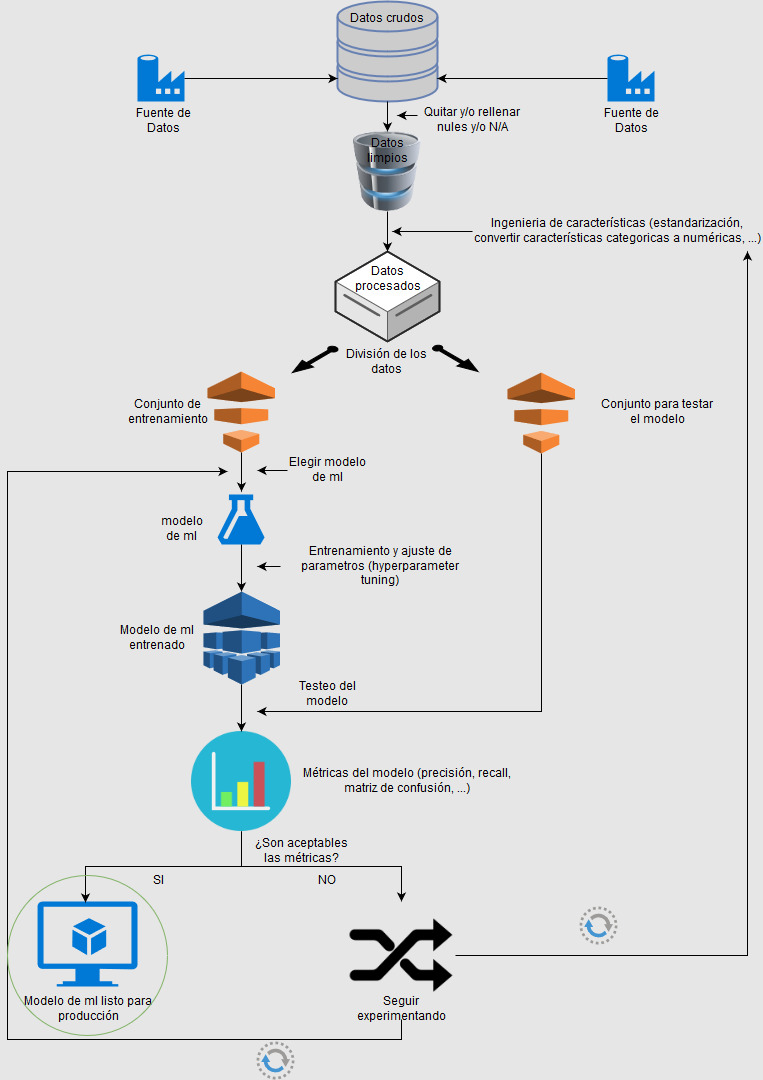
\includegraphics[width=\textwidth]{C:/Users/David/Desktop/TFG/TFGLatex/imagenes/ml_pipeline.jpg}
  \caption[\textit{Machine learning pipeline}]{Diagrama de flujo de un proyecto de \textit{machine learning}}
  \label{ml_pipeline}
\end{figure}

\clearpage


\chapter[Implementación paralela]{Implementación paralela de algoritmos}\label{chap:implementacion_paralela}
En este capítulo se implementarán algunos de los algoritmos más populares de \textit{machine learning} 
pero con un enfoque distribuido, con el fin de minimizar los tiempos de ejecución a medida que
el \textit{dataset} se vuelve más grande.
Cada sección consistirá en explicar de una manera breve y concisa la problemática a estudiar, 
el algoritmo a desarrollar y la publicación del código fuente del algoritmo en paralelo.
\newline

Para comenzar, vamos a establecer una serie de convenciones para la notación, con el fin de explicar
las matemáticas que hay detrás de los algoritmos de \textit{machine learning}.\\
El numero total de datos de entrenamiento se marcara con la letra $m$, mientras que es numero total
de características de los datos se denotara con la letra $n$.\\
Un dato de entrenamiento sera un vector fila donde cada componente del vector será una característica
de dicho dato. A cada dato del conjunto de entrenamiento se le denotara con la letra $x$ y un 
superíndice, mientras que las características se denotaran con la letra $x$ y subíndices.\\ 
En caso de que el dato lleve aparejado una clase a la que pertenece, ésta será denotada con la letra 
$y$. Así pues, para un primer ejemplo de entrenamiento (supervisado) sería:
$$ x^{(1)}=(\underbrace{x^{(1)}_1, x^{(1)}_2, \cdots, x^{(1)}_n}_{\text{n características}}) \in \mathds{R}^n; \>
   y^{(1)} \in \mathds{R} $$

Al conjunto total de datos lo denotaremos con la letra $X$ que representará la matriz que contiene
todos los datos de entrenamiento, donde cada ejemplo será un vector fila de la matriz.
La letra $y$ será un vector columna conteniendo las clases de sus respectivos datos (aparejados por el índice), 
por lo que a la fila $i$-ésima de la matriz le corresponde la clase $i$-ésima del vector $y$.
Si estamos hablando de un problema de aprendizaje no supervisado, no tendría sentido hablar de las clases 
aparejadas a cada dato, con lo cual el vector $y$ no existiría.\\
A modo de ejemplo, el conjunto de entrenamiento para un problema de aprendizaje supervisado quedaría así:

$$
X = \left(\begin{array}{ccc}
    \textemdash & x^{(1)} & \textemdash \\
    \textemdash & x^{(2)} & \textemdash \\
     & \vdots &  \\
    \textemdash & x^{(m)} & \textemdash \\
\end{array}\right)
%
=
  \left(\begin{array}{ccccc}
    x^{(1)}_1 & x^{(1)}_2 & x^{(1)}_3 & \cdots & x^{(1)}_n \\
    x^{(2)}_1 & x^{(2)}_2 & x^{(2)}_3 & \cdots & x^{(2)}_n \\
    \vdots & \vdots & \vdots & \ddots & \vdots \\
    x^{(m)}_1 & x^{(m)}_2 & x^{(m)}_3 & \cdots & x^{(m)}_n \\
\end{array}\right)
%
;
y = \left(\begin{array}{c}
    y^{(1)} \\
    y^{(2)} \\
    \vdots \\
    y^{(m)} \\
\end{array}\right)
$$

De manera análoga si hubiera que hacer distinción entre los datos de entrenamiento y los datos de test, 
se denotarán $X_{train}, y_{train}$ y $X_{test}, y_{test}$.


\section{Aprendizaje supervisado}
En el aprendizaje supervisado necesitamos que cada dato de entrenamiento lleve aparejado una clase 
a la que pertenece. De esta manera nuestro algoritmo intentara adaptarse a los datos lo mejor 
posible corrigiendo los errores en función de la clase real de cada ejemplo.
En esta sección se estudiaran los algoritmos de Regresión Lineal y \textit{NaiveBayes}.
\subsection{Regresión lineal}
La \textbf{Regresión Lineal}\index{Regresión!Lineal} es un potente algoritmo de \textit{machine learning} que 
permite predecir el comportamiento de una variable dependiente $y \in \mathds{R}$ a partir de los 
valores de la variable independiente $x \in \mathds{R}^n$.
El modelo se puede expresar como una ecuación o recta de regresión 
$$h_{\theta}(x) = \theta^T x = \theta_0 + \theta_1 x_1 + \cdots + \theta_n x_n$$
de la cual se debe ajustar el parámetro desconocido $\theta \in \mathds{R}^n$ para que el error 
de las predicciones sea el menor posible.

Dicho error viene representado por la función de perdida cuadrática
$$J(\theta) = \frac{1}{2m} \sum_{i=1}^{m}(\theta^Tx^{(i)} - y^{(i)})^2$$
donde $\theta^Tx^{(i)}$ representa el valor predecido para el ejemplo $i$-ésimo del \textit{dataset}, y la variable 
$y^{(i)}$ representa el valor real del ejemplo $i$-ésimo.

Gráficamente, en $\mathds{R}^2$, el problema consiste en ajustar lo mejor posible una recta a los 
puntos que representan los ejemplos de entrenamiento

\begin{figure}[h]
  \centering
  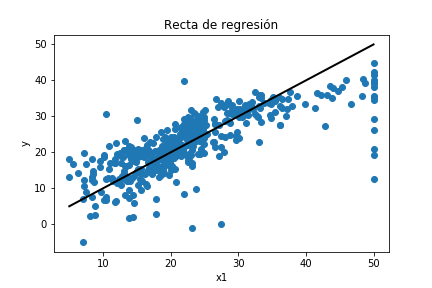
\includegraphics[width=\textwidth]{C:/Users/David/Desktop/TFG/TFGLatex/imagenes/recta_regresion.png}
  \caption[Regresión lineal en $\mathds{R}^2$]{Recta de regresión}
  \label{recta_regresion}
\end{figure}

\noindent \textbf{Gradiente de descenso}\\
Uno de los algoritmos mas populares de optimización de funciones es el algoritmo del Gradiente 
de Descenso\index{Gradiente de descenso} 
(\href{https://en.wikipedia.org/wiki/Gradient_descent}{\textit{Gradient Descent}}).
Este algoritmo consiste en actualizar los pesos o variables $\theta_i \enskip \forall i=1, \cdots, n$ de 
manera que con cada iteración se vaya reduciendo el error $J(\theta)$.
Las actualizaciones en cada iteración están dadas por la siguiente fórmula~\cite{DBLP:books/lib/Bishop07}

\begin{equation}
\theta := \theta - \alpha \frac{1}{m} \sum_{i=1}^{m}(h_{\theta}(x^{(i)}) - y^{(i)})x^{(i)}
\end{equation}

donde $\alpha$ es un parámetro que controla el salto que se produce en cada iteración del algoritmo, 
también denominado tasa de aprendizaje o \textit{learning rate}.
A valores pequeños del parámetro la iteración se vuelve mas lenta pero mas segura, por el contrario, 
valores grandes del parámetro producen que el algoritmo se acelere de manera considerable pero a costa 
de correr el riesgo de que incluso no llegue a converger.

\clearpage

Una manera lógica de paralelizar este computo es dividir el trabajo en el conjunto de entrenamiento 
de tal manera que cada máquina trabaje sobre un cierto numero de ejemplos de entrenamiento y no 
sobre el conjunto total.
Supongamos que nuestro conjunto de entrenamiento $X$ tiene un total de $m=4 \cdot 10^8$ de ejemplos.
Una iteración del algoritmo de descenso de gradiente tiene que recorrer todos los ejemplos y realizar 
un calculo con cada uno de ellos, sin embargo, definamos lo siguiente:
$$ temp^{(1)} = \sum_{i=1}^{10^8}(h_{\theta}(x^{(i)}) - y^{(i)})x^{(i)} $$
Este calculo sería realizado en una máquina (notese que solo utiliza un cuarto del \textit{dataset} original) 
de tal manera que esta máquina en particular solo contendría un cuarto del calculo total a realizar.
De manera análoga definimos
$$ temp^{(2)} = \sum_{i=10^8+1}^{2 \cdot 10^8}(h_{\theta}(x^{(i)}) - y^{(i)})x^{(i)} $$
que sería el calculo a realizar por la segunda máquina.
Así sucesivamente, hemos dividido el trabajo en 4 porciones que se desarrollan de manera totalmente 
independiente y paralela.\\
Sin embargo, el calculo de una iteración del gradiente de descenso no 
acaba aquí, ya que necesitamos combinar los resultados de estas cuatro máquinas.\\
Esto de nuevo en sencillo, ya que un ultimo cálculo requeriría juntar las cuatro porciones de la 
siguiente manera:
$$ \theta := \theta - \alpha \frac{1}{4 \cdot 10^8}(temp^{(1)} + temp^{(2)} + temp^{(3)} + temp^{(4)}) $$
De manera gráfica, para una paralelización en $n$ partes, cada partición de los datos se alojaría en un nodo
como un bloque de datos el cual sería procesado y luego enviado a través de la red a un nodo que recibiría
todas las partes y haría la agregación o combinación de los resultados.

\begin{figure}[h]
  \centering
  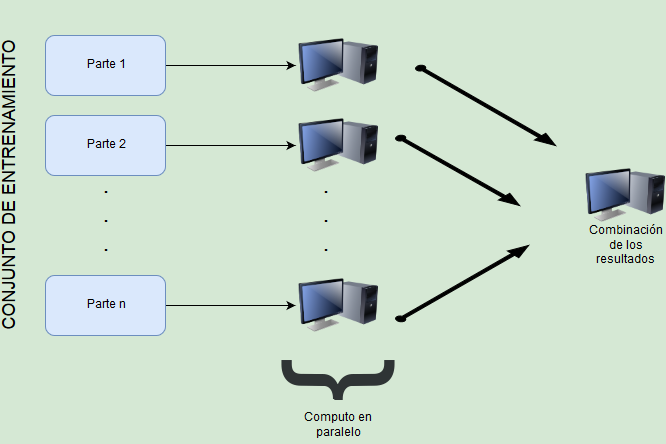
\includegraphics[width=\textwidth]{C:/Users/David/Desktop/TFG/TFGLatex/imagenes/computo_paralelo.png}
  \caption[División de los datos en el gradiente de descenso]
          {Computo en paralelo y agregación de los datos}
  \label{computo_paralelo}
\end{figure}

\newpage

\subsubsection*{Código \textit{Spark} Regresión lineal}
\lstinputlisting[caption=LinearRegression.py, language=Python, firstline=8]
                {C:/Users/David/Desktop/TFG/implementaciones/LinearRegression.py}

\begin{lstlisting}[language=bash, numbers=none]
$ spark-submit --master yarn-client LinearRegression.py
\end{lstlisting}

\clearpage

\subsection{Naive-Bayes}
Un clasificador \textbf{NaiveBayes}\index{NaiveBayes} es un clasificador probabilístico que se apoya en el 
\textit{Teorema de Bayes} para clasificar las entradas.
Es un modelo que asume que las características de las variables de entrada son independientes 
entre sí, esto es, el valor de una cierta variable no influye para nada en el valor de otra.\\
La idea general detrás del algoritmo es calcular la media y la varianza de cada clase y cada característica.
Una vez realizado ésto, se pueden utilizar los valores obtenidos para predecir la clase de un nuevo 
dato de entrada. El modelo lo etiquetará con la clase que mas se parezca de las vistas en el 
conjunto de entrenamiento.
\newline

Como se ha mencionado anteriormente, el algoritmo utiliza el teorema de Bayes para asignar la probabilidad de
un suceso condicionado a la ocurrencia de otro. En el ejemplo explicado mas abajo dichos sucesos serían la
probabilidad a priori y a posteriori de ser hombre o mujer.
%\newline

\begin{theorem}[Teorema de Bayes]\index{Teorema de Bayes}
  Sean ${A_1, A_2, \cdots, A_n}$ sucesos con $P(A_i) \neq 0 \quad \forall i=1, 2, \cdots, n$. 
  Sea $B$ un suceso cualquiera del que se conocen $P(B|A_i) \quad \forall i=1, 2, \cdots, n$.
  Entonces:
  {\fboxsep 8pt\fboxrule 1pt
  \begin{equation*}
  \fbox{$ P(A_i|B) = \frac{P(B|A_i) \cdot P(A_i)}{P(B)} $}
  \end{equation*}
  }
%  $$ P(A_i|B) = \frac{P(B|A_i) \cdot P(A_i)}{P(B) $$
\end{theorem}

Supongamos que queremos clasificar a una persona en hombre o mujer a través de características como 
la altura, el peso y el numero de pie. Aquí nuestras características serian $n=3$ y el objetivo 
sería predecir la variable $y=0$ si es hombre o $y=1$ si es mujer.
A partir de un \textit{dataset} de ejemplos etiquetados con hombre o mujer,
el concepto de aprendizaje para el algoritmo  sería calcular la media y la varianza 
de la altura, el peso y la talla de pie de todos los hombres y mujeres por separado.
Con estos datos, estamos en disposición de calcular la probabilidad a posteriori y las probabilidades 
condicionadas que servirán al algoritmo para realizar sus predicciones.

\begin{figure}[!htpb]
  \centering
  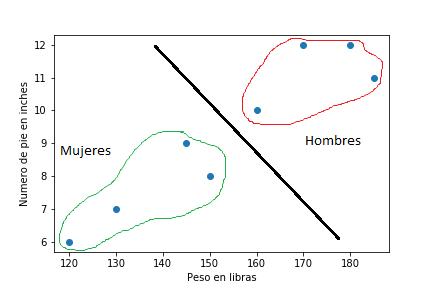
\includegraphics[width=0.5\textwidth]{C:/Users/David/Desktop/TFG/TFGLatex/imagenes/naiveBayes_men_women.png}
  \caption[Naive Bayes clasificación]{Clasificación entre hombres y mujeres}
  \label{men_women_boundary}
\end{figure}

Debido a la simplicidad de los cálculos que usa para entrenarse, \textit{NaiveBayes} se desempeña muy bien 
en conjuntos de datos muy grandes dando lugar a modelos muy precisos.\\
Sin embargo, como todo modelo, tiene sus ventajas e inconvenientes que hacen de \textit{NaiveBayes} un modelo 
propicio para unos determinados tipos de problemas.

\begin{itemize}
  \item Ventajas:
  \begin{enumerate}
    \item Funciona muy bien en problemas multiclase. Dado un dato, es rápido y fácil predecir su clase.
    \item Asumiendo la independencia de las clases, un clasificador \textit{NaiveBayes} obtiene un mejor 
    desempeño comparado con otros métodos como la regresión logística, además necesita menos datos 
    de entrenamiento.
  \end{enumerate}
  \item Inconvenientes:
  \begin{enumerate}
    \item Si en los datos de test hay una característica nunca antes vista en los datos de 
    entrenamiento, el modelo le asignará una probabilidad de 0 y será incapaz de hacer una predicción.
    Esto es conocido como frecuencia cero o \textit{zero frequency}.
    \item En la vida real, es casi imposible encontrar un \textit{dataset} donde todas las características 
    sean completamente independientes unas de las otras.
  \end{enumerate}
\end{itemize}

\subsubsection*{Código MapReduce NaiveBayes}
\lstinputlisting[caption=NaiveBayes.py, language=Python, firstline=10]
                {C:/Users/David/Desktop/TFG/implementaciones/NaiveBayes.py}
                  
\begin{lstlisting}[language=bash, numbers=none]
$ python NaiveBayes.py <input_file> [-r hadoop]
\end{lstlisting}

Para el desarrollo de este código se ha elegido el \textit{framework MapReduce} debido a que la arquitectura del
algoritmo es altamente paralelizable, esto es consecuencia de la asociatividad de las operaciones que se calculan.\\
En la fase \textit{map} se parsea la línea y se separa en campos (divididos por coma), las características se 
asignan a la variable $x$ y el último campo es la clase, asignada a la variable $y$.\\
Como clave se emite una tupla que tiene por valor la clase ($y$) y la posición del campo ($i$), mientras que
como valor se emite otra tupla que contiene el valor del propio campo ($x[i]$) y un 1 que servirá para hacer
un conteo de los datos. Esta elección ha sido así ya que se consigue la máxima paralelización al dividir las 
claves (\textit{key}) en tantas como campos tengan los registros.\\
En la fase \textit{reduce} se crean 3 variables: $m$, $sum\_features$ y $sum\_features\_squared$. La primera sirve
para hacer la agregación del conteo de registros, la segunda y tercera sirven como variables auxiliares para 
posteriormente calcular la media $\mu_j$ y la varianza $\sigma^2$.
                    
\clearpage


\section{Aprendizaje no supervisado}
En el aprendizaje no supervisado es el propio algoritmo el que debe sacar los patrones de 
comportamiento de todo el conjunto de datos.
En esta sección se estudiaran los algoritmos de Detección de anomalías y \textit{K-Means}.
\subsection{Sistema de detección de anomalías}
Un sistema de detección de anomalías es un software capaz de detectar comportamientos anómalos a 
partir de comportamientos previamente establecidos como normales.
La base de este modelo es la distribución Gaussiana y requiere que nuestro conjunto de 
datos tenga variables o características que se distribuyan según una normal de media $\mu$ y  
varianza $\sigma^2$, es decir, $\mathcal{N}(\mu, \sigma^2)$.\\
Este modelo es usado frecuentemente en detección de intrusos de una red, monitorización de las 
máquina de un data center, detección de fraude en el uso de tarjetas de crédito...
\newline

La distribución Gaussiana\index{Distribución!Gaussiana} (o distribución normal\index{Distribución!Normal}) 
es una distribución de probabilidad que aparece con mucha frecuencia en fenómenos reales, lo cual es ideal 
para poder modelar estos fenómenos desde un punto de vista estadístico.

\begin{figure}[h]
  \centering
  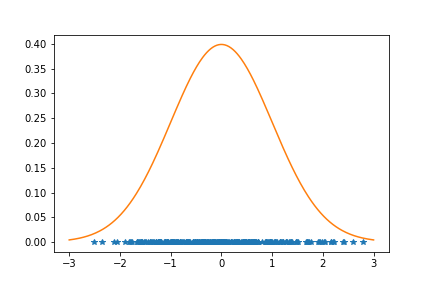
\includegraphics[scale=0.6]{C:/Users/David/Desktop/TFG/TFGLatex/imagenes/normal_01.png}
  \caption[$\mathcal{N}(0,1)$]{Distribución normal de media 0 y desviación típica 1}
  \label{normal_01}
\end{figure}

Esta función será nuestro punto de partida para construir nuestro modelo, el cual asume que las 
características de los datos siguen dicha distribución, es decir, 
$\forall j=1,\cdots,n; \quad x_j \sim \mathcal{N}(\mu_j, \sigma_j^2)$.\\

El objetivo es modelizar una función que denotaremos $p(x)$, la cual, dado un ejemplo nos devuelva la 
probabilidad de que dicho ejemplo sea anómalo. Más adelante se definirá esta función de manera 
concreta.\\
Lo primero que debemos hacer es calcular las medias y varianzas de cada característica de nuestros 
ejemplos de entrenamiento (matriz $X$), esto nos da una serie de parámetros 
$\mu = (\mu_1, \ldots, \mu_n) $ y 
$\sigma^2 = (\sigma_1^2, \ldots, \sigma_n^2) $ 
que se utilizaran posteriormente para predecir la probabilidad de que un nuevo dato sea anómalo. 
Más concretamente:
$$ \mu_j = \frac{1}{m}\sum_{i=1}^{m}x_j^{(i)} \quad 
   \sigma_j^2 = \frac{1}{m}\sum_{i=1}^{m}(x_j^{(i)} - \mu_j)^2 $$

\noindent Una vez que tenemos nuestros parámetros calculados ya podemos definir $p(x;\mu,\sigma^2)$ como:
$$ p(x;\mu,\sigma^2) = \frac{1}{\sqrt{2\pi}\sigma}e^{-\frac{1}{2}\frac{x-\mu}{\sigma^2}^2}$$
Esta fórmula nos da la probabilidad de que un valor de una determinada característica se 
comporte de manera anómala.

\clearpage

Una vez calculadas todas las curvas gaussianas para cada característica del \textit{dataset}, definimos $p(x)$ como:
$$ p(x) = \prod_{j=1}^n p(x_j;\mu_j,\sigma_j^2)= p(x_1; \mu_1, \sigma_1^2) \cdots  p(x_n; \mu_n, \sigma_n^2)$$
La función $p(x)$ se comporta como un detector de irregularidades ya que si alguna de las funciones 
$p(x_j;\mu_j,\sigma_j^2)$ para cierto $j$ arroja un valor fuera de lo normal, este quedará reflejado 
en el valor final de $p(x)$.\\
Llegados a este punto, debemos establecer un cierto umbral $\epsilon$ que nos marque la frontera 
para considerar un ejemplo como normal o anómalo, es decir, marcaremos un ejemplo $x$ como anómalo si 
$p(x)<\epsilon$ y será considerado normal si por el contrario $p(x)>=\epsilon$.
Esta elección del parámetro $\epsilon$ no es algo universal sino que depende del problema en cuestión 
(\autoref{circles_plot}) y el \textit{dataset} utilizado para modelar $p(x)$.
Existen ciertas directrices así como reglas generales para una buena elección de 
$\epsilon$\footnote{\url{https://www.coursera.org/learn/machine-learning/lecture/Mwrni/developing-and-evaluating-an-anomaly-detection-system}}, pero están fuera de los objetivos de este documento.
\newline
Gráficamente, la función $p(x)$ establece una bola n-dimensional con un cierto centro 
y radio que dependerá del epsilon elegido y el \textit{dataset} utilizado. Toda representación 
de un ejemplo en el espacio $\mathds{R}^n$ que quede dentro de dicha bola, será considerado normal, 
si por el contrario dicha representación queda fuera de la bola, entonces será considerado una 
anomalía.

\begin{figure}[h]
  \centering
  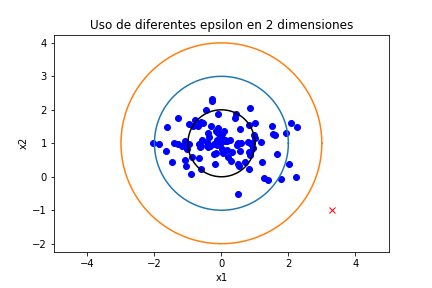
\includegraphics[scale=0.6]{C:/Users/David/Desktop/TFG/TFGLatex/imagenes/circles_plot.png}
  \caption[Ejemplo de anomalía]{Ejemplo de anomalías para distintos valores de $\epsilon$}
  \label{circles_plot}
\end{figure}

En la figura los valores se distribuyen según
$x1 \sim \mathcal{N}(0, 1); \quad x2 \sim \mathcal{N}(1, 0.5)$.
Los círculos concéntricos representan la elección de distintos valores del parámetro $\epsilon$ ,
centrados en el punto $\mu=(\mu_1, \mu_2)=(0, 1)$.
Si tomamos como referencia el circulo más grande, la $x$ marcada en rojo sería un ejemplo anómalo 
en ese conjunto de datos

\newpage  
  
\subsubsection*{Código MapReduce para el computo de la media y la varianza}
  
\lstinputlisting[caption=ComputeMeanVar.py, language=Python, firstline=10]
                {C:/Users/David/Desktop/TFG/implementaciones/ComputeMeanVar.py}

\begin{lstlisting}[language=bash, numbers=none]
$ python ComputeMeanVar.py <input_file> [-r hadoop]
\end{lstlisting}

La elección de \textit{MapReduce} para desarrollar este algoritmo ha sido debido a que para calcular la media y 
la varianza de un conjunto de datos, solo es necesario un escaneo completo del \textit{dataset}. Como se ve
gráficamente en la \autoref{mapReduce_wordcount}, en la fase map se produce el parseo de los datos donde cada línea
se divide separando los campos por coma (\textit{,}). Los valores emitidos son: la posición del campo ($i$) como clave
y el valor del campo ($fields[i]$) y un 1 como valor. Este 1 sirve para hacer un conteo de los datos en la fase 
\textit{reduce}.\\
En dicha fase \textit{reduce}, se itera sobre los valores recibidos en la fase \textit{map} y se descompone el calculo
de la media en 2 variables, aparte de crear otra variable $m$ que será un contador de los registros totales por cada campo.
Una vez terminado la iteración del \textit{for}, se utilizan las variables \textit{sum\_features} y 
\textit{sum\_features\_squared} para calcular la media $\mu_j$ y la varianza $\sigma^2$.
\newline

Para el despliegue de la aplicación, se puede hacer de manera local (usado principalmente para depuración del código)
o de manera distribuida haciendo uso de un \textit{cluster Hadoop} para que la computación se produzca en paralelo
(\textit{-r hadoop}). Este último modo de despliegue sube el archivo \path{input_file} a \textit{HDFS} para su 
posterior ejecución con \textit{MapReduce}. También se puede indicar que el archivo ya se encuentra en \textit{HDFS}
poniendo delante el prefijo de hdfs en el path: \path{hdfs://<input_file_in_hdfs>}
  
\newpage

\subsection{K-Means}
\textbf{\textit{K-Means}}\index{K-Means} es uno de los algoritmos de \textit{clusterización}\index{Clusterización} más 
extendidos y usados en la actualidad. La idea principal del algoritmo es agrupar los datos de entrada 
en distintos conjuntos o \textit{clusters}\footnote{Notese que no se debe confundir el uso de la 
palabra \textit{cluster} para hacer referencia a un \textit{cluster} de maquinas, o cuando se usa 
para referirnos a un conjunto de datos agrupados.} 
coherentes, esto es, los puntos dentro de una mismo \textit{cluster} son más parecidos entre sí 
que los puntos de otro \textit{cluster} cualquiera.
\newline

Nuestros datos de entrada son puntos $x^{(i)} \in \mathds{R}^n$ y un cierto numero $k \in \mathds{N}$ de 
\textit{clusters} en los que vamos a agrupar nuestros datos.\\
Comenzamos estableciendo $k$ puntos en lugares aleatorios de nuestros datos, estos puntos serán los 
centros de los \textit{clusters} $c_1, c_2, \cdots, c_k$, y los llamaremos \textit{centroides}\index{Centroides}.
Una vez hecho esto, el algoritmo recorrerá cada punto $x_i$ y encontrará el centroide $c_j$ más 
cercano (en términos de la distancia euclídea) a nuestro punto. Por lo cual, al punto $x_i$ se le 
asigna el \textit{cluster} $j$.\\
Una vez que tengamos todos los puntos asignados a sus respectivos centroides más cercanos, actualizamos 
los centroides con la media de todos los puntos que pertenecen al \textit{cluster} de dicho centroide.\\
Las iteraciones del algoritmo se detendrán cuando en dos iteraciones sucesivas ninguno de los puntos 
sea asignado a otro \textit{cluster} distinto al anterior o cuando la norma del vector que componen 
la resta de los centroides de dos iteraciones consecutivas sea menos que un cierto $\epsilon$ 
prefijado.
\newline

\noindent \textbf{Pasos del algoritmo K-Means}:
\begin{enumerate}
  \item[] \textbf{Input}: Puntos en $\mathds{R}^n$ y un numero $k \in \mathds{N}$ de \textit{clusters}
  en los que agrupar nuestros datos.
  \item Insertar $k$ centroides $c_1, c_2, \cdots, c_k$ en localizaciones aleatorias.
  \item Calcular la distancia entre cada punto $x^{(i)}$ y cada centroide $c_i$.
  \item Asignar a cada punto $x^{(i)}$ al \textit{cluster} cuya distancia al centroide sea menor 
        que la distancia al resto de centroides.
  \item Recalcular los nuevos centroides usando la formula $c_i = \frac{1}{m_j} \sum_{j=1}^{m_i}x^{(i)}$ 
        donde $m_i$ es el número de puntos que pertenecen al \textit{cluster} $i$ y $x^{(i)}$ son 
        todos los puntos de dicho cluster, más concretamente \\
        $x^{(i)} \in \{ p \in \mathds{R}^n \, | \, d(p, c_j) < d(p, c_s) \, \forall s \in 1, \cdots, k; s \neq j \}$.
  \item Calcular la norma entre los centroides anteriores y los nuevos centroides \\
        $ ||(c_1^i, c_2^i, \cdots, c_k^i) - (c_1^{i-1}, c_2^{i-1}, \cdots, c_k^{i-1})||_{\infty} $ 
        donde el superíndice $i$ indica la iteración $i$-ésima.
  \item Si dicha norma es menor que un cierto $\epsilon$ prefijado entonces parar (se ha llegado a la convergencia), 
        en caso contrario volver al paso $2$.
  \item[] \textbf{Output}: $k$ centroides $c_1, c_2, \cdots, c_k$.
\end{enumerate}

\begin{figure}[htp]
  \centering
  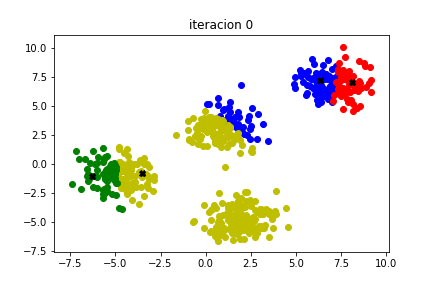
\includegraphics[width=.3\textwidth]{C:/Users/David/Desktop/TFG/TFGLatex/imagenes/kmeans_imagen0.png}\quad
  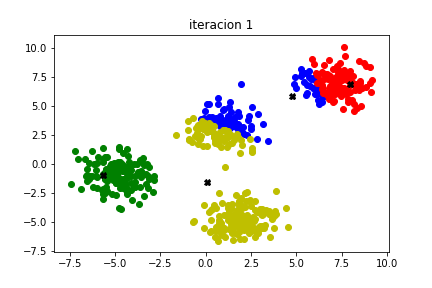
\includegraphics[width=.3\textwidth]{C:/Users/David/Desktop/TFG/TFGLatex/imagenes/kmeans_imagen1.png}\quad
  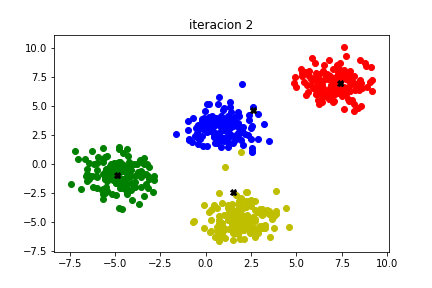
\includegraphics[width=.3\textwidth]{C:/Users/David/Desktop/TFG/TFGLatex/imagenes/kmeans_imagen2.png}

  \medskip

  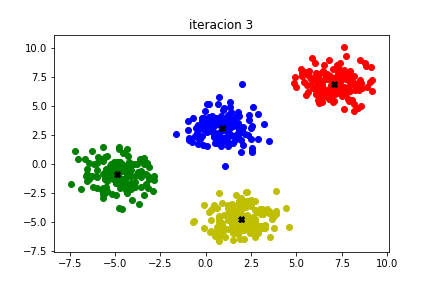
\includegraphics[width=.3\textwidth]{C:/Users/David/Desktop/TFG/TFGLatex/imagenes/kmeans_imagen3.png}\quad
  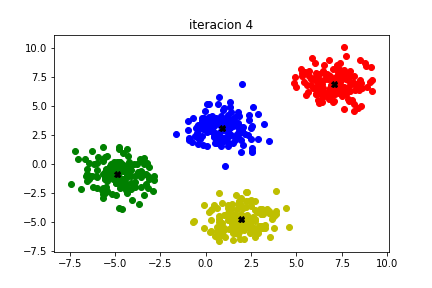
\includegraphics[width=.3\textwidth]{C:/Users/David/Desktop/TFG/TFGLatex/imagenes/kmeans_imagen4.png}

  \caption{Iteraciones del algoritmo k-means}
  \label{kmeans_iteraciones} % para las hyperreferencias
\end{figure}

\newpage

\subsubsection*{Código \textit{Spark} para el algoritmo de \textit{K-Means}}

\lstinputlisting[caption=KMeansSpark.py, language=Python, firstline=8, lastline=72]
                {C:/Users/David/Desktop/TFG/implementaciones/KMeansSpark.py}

\clearpage
Con el fin de testar el código anteriormente escrito:

\lstinputlisting[caption=KMeansMain, language=Python, firstline=74]
                {C:/Users/David/Desktop/TFG/implementaciones/KMeansSpark.py}

\begin{lstlisting}[language=bash, numbers=none]
$ # master puede ser local[*] o yarn-client
$ spark-submit --master yarn-client KMeansSpark.py
\end{lstlisting}

Para el desarrollo de este código se ha elegido el \textit{framework Spark} debido principalmente a que el algoritmo
de \textit{K-Means} es un algoritmo iterativo sobre los mismos datos para realizar los computos. Debiado a la capacidad
de \textit{Spark} de cachear los datos en memoria, los tiempos de ejecución se reducirán considerablemente.
\newline

Los datos de entrada del algoritmo es un \textit{RDD} que contiene como registros objetos \textit{numpy arrays}.
Lo primero que se hace es cachear los datos en memoria y a continuación inicializar los centroides en posiciones
aleatoria de los datos de entrada.\\
Dentro del bucle \textit{while}, la variable \textit{points\_clusterized} contiene un mapeo de los datos originales
a una tupla que contiene el centroide más cercano al punto $p$ en cuestión y un 1 que permite realizar posteriormente
el conteo de los puntos totales. La variable \textit{clusters\_set} realiza una agregación que suma los puntos de
entrada y los unos anteriores para realizar la media de cada \textit{cluster} de puntos.\\
La variable \textit{new\_centroids} realiza un mapeo de los valores para calcular la división 
de la suma de los puntos y el conteo, de esta manera se obtienen los nuevos centroides que se guardan en la variable
\textit{new\_centroids}. Por último, se calcula la distancia entre los nuevos centroides y los anteriores con el fin
de calcular la distancia para el criterio de parada (del bucle \textit{while}).\\
Las iteraciones se detendrán cuando la distancia entre los centroides de dos iteraciones consecutivas sea menor
que un cierto $\epsilon$ prefijado (o cuando se superen las máximas iteraciones permitidas).
\newline

El modo de despliegue de la aplicación depende de si como \textit{master} ponemos que se ejecute en local 
(\textit{local[*]}) o en distribuido (\textit{yarn-client}). El primero no distribuye ningún cálculo en absoluto
mientras que el segundo es un cliente del gestor de recursos del \textit{cluster}, \textit{YARN}.

\newpage
